\chapter{Bose-Einstein condensation} 
\label{chapter3}
%===============================================================================================
\section{Historical foundation} %TO DO!! Check the title 
The concept of \textit{Bose--Einstein condensation} (BEC) originates from the early development of quantum statistics in the 1920s.  
In 1924, \textit{Satyendra Nath Bose} introduced a new counting rule for indistinguishable photons, leading to what is now known as \textit{Bose--Einstein statistics}.  
Shortly after, \textit{Albert Einstein} extended Bose's formalism to a gas of material particles obeying the same statistics (bosons).  
Einstein predicted that, below a certain critical temperature \( T_c \), a macroscopic fraction of these particles would accumulate in the lowest quantum state of the system, producing a new phase of matter characterized by long-range quantum coherence\footnote{%
Long-range quantum coherence refers to the property whereby the quantum phases of individual particles become correlated across macroscopic distances.  
As a result, the entire system can be described by a single complex wavefunction with a well-defined global phase.}.  
For decades, this prediction remained purely theoretical.

Only in 1995 was Bose--Einstein condensation realized experimentally in dilute atomic gases by \textit{Cornell} and \textit{Wieman} (rubidium) and by \textit{Ketterle} (sodium), achievements that earned them the Nobel Prize in Physics in 2001.  
These experiments confirmed the existence of a macroscopic quantum state at ultralow temperatures, with a sharply peaked momentum distribution indicating the population of a single ground-state wavefunction.  
From a physical standpoint, the condensate can be viewed as a collection of bosons occupying the same single-particle state, described by a common wavefunction, below a critical temperature \( T_c \).  


\section{Bose--Einstein distribution}
The quantum statistical behaviour of bosons differs fundamentally from that of classical particles.\\
Because bosons are indistinguishable and do not obey the Pauli exclusion principle\footnote{Formulated by Wolfgang Pauli in 1925, the Pauli exclusion principle states that two identical fermions cannot occupy the same quantum state simultaneously. This rule follows from the antisymmetric nature of the fermionic wavefunction under particle exchange.}, any number of them can occupy the same quantum state.
For a system in thermal equilibrium, the average occupation number of a single-particle energy level \( \varepsilon_i \) is given by the \textit{Bose--Einstein distribution}\footnote{Throughout this work, the same function will also be denoted as $f(\varepsilon)$.}:
\begin{equation}
    \langle n_i \rangle = \frac{1}{e^{\beta(\varepsilon_i - \mu)} - 1},
    \label{eq:BE_distribution}
\end{equation}
where \( \beta = 1/(k_B T) \) is the Boltzmann factor\footnote{More generally, \( \beta \) is defined as the \textit{thermodynamic beta}, a numerical quantity related to the system’s temperature that establishes a connection between the statistical and thermodynamic descriptions of a system.} and \( \mu \) is the chemical potential.  

\begin{figure}[H]
    \centering
    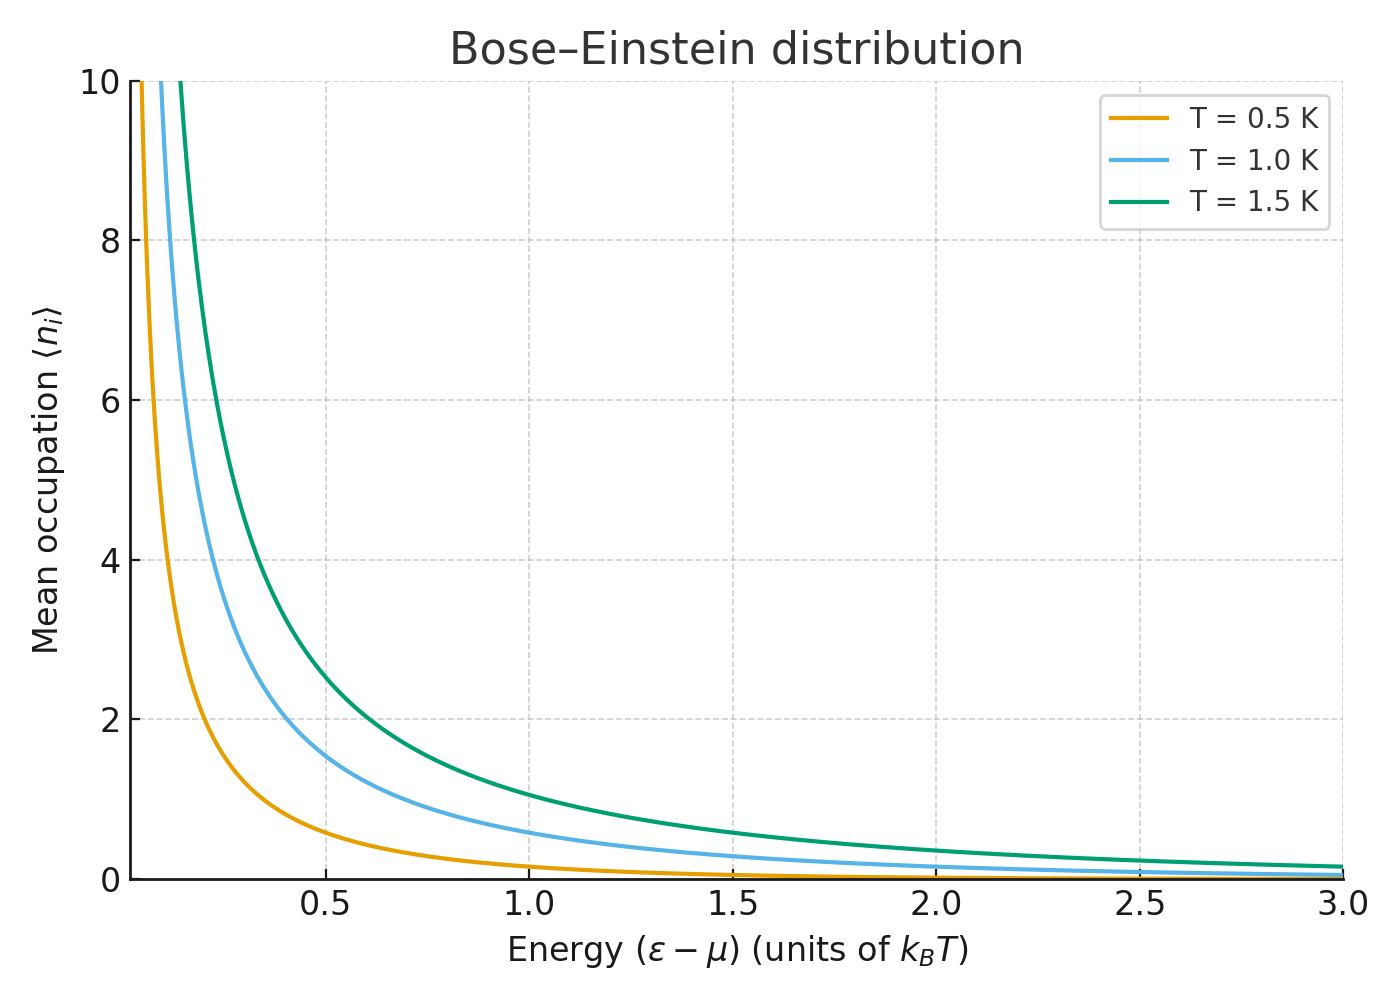
\includegraphics[scale= 0.6]{Chapters/Chapter_2/Images/1_Bose_einstein.png}
    \caption{Bose-Einstein distribution: the mean occupation number \( \langle n_i \rangle \) is shown as a function of the normalized energy \( (\varepsilon - \mu)/(k_B T) \) for three temperatures.}
    \label{Figure 4 - Bose_Einstein_distribution}
\end{figure}

As the temperature decreases, the system departs from classical behaviour.  
The chemical potential \( \mu \) increases towards zero (\( \mu \to 0^- \)), and the denominator in Eq.~\eqref{eq:BE_distribution} becomes small for low-energy states.  
When \( \varepsilon \approx \mu \), the exponential approaches unity and the occupation number diverges:
\[
    \langle n_i \rangle \rightarrow \infty.
\]
This divergence indicates that an increasingly large fraction of bosons accumulate in the lowest-energy state of the system. At sufficiently low temperature, this results in a macroscopic occupation of the ground state. In the extreme limit \( T \to 0 \), all particles occupy the ground state.

\subsection*{Classical limit}
In the limit of high temperature or low density, the system behaves classically.  
When the term \( \beta(\varepsilon - \mu) \gg 1 \), the exponential dominates over unity, so that:
\[
    e^{\beta(\varepsilon - \mu)} \gg 1 \quad \Rightarrow \quad 
    \langle n_i \rangle \approx e^{-\beta(\varepsilon_i - \mu)}.
\]
This corresponds to the \textit{Maxwell--Boltzmann distribution}, which governs classical particles.  
In this regime, the mean occupation number of each state is small, and quantum statistical effects can be neglected.


\paragraph{Comparison with the Maxwell--Boltzmann distribution.}
To illustrate the difference between classical and quantum statistics, we consider a simple model system of \( N = 6 \) indistinguishable particles distributed among \( 9 \) discrete energy levels.  
Each level \( \varepsilon_i \) is separated by a fixed energy spacing, and the system is assumed to be in thermal equilibrium at temperature \( T \).  
For this small system, the average occupation numbers predicted by the \textit{Maxwell--Boltzmann} and \textit{Bose--Einstein} distributions can be compared directly.  
The results are summarized in Table~\ref{tab:BE_MB_comparison}.  

\begin{table}[H]
    \centering
    \begin{tabular}{ccc}
        \hline
        \textbf{Energy level} & \textbf{Maxwell-Boltzmann} $\langle n_{\mathrm{MB}}\rangle$ & \textbf{Bose-Einstein} $\langle n_{\mathrm{BE}}\rangle$ \\
        \hline
        0 & 2.143 & 2.269 \\
        1 & 1.484 & 1.538 \\
        2 & 0.989 & 0.885 \\
        3 & 0.629 & 0.538 \\
        4 & 0.378 & 0.269 \\
        5 & 0.210 & 0.192 \\
        6 & 0.105 & 0.115 \\
        7 & 0.045 & 0.077 \\
        8 & 0.015 & 0.038 \\
        9 & 0.003 & 0.038 \\
        \hline
    \end{tabular}
    \caption{
    Comparison between the Maxwell--Boltzmann and Bose--Einstein distributions for a system of \( N = 6 \) particles and \( 9 \) discrete energy levels at temperature \( T \). \\Numerical values adapted from Blatt~\cite{blatt1992}.
    }
    \label{tab:BE_MB_comparison}
\end{table}

The data show that the Bose--Einstein distribution yields a larger occupation of the lowest energy states compared to the Maxwell--Boltzmann case. This occurs because, unlike classical particles, bosons can accumulate in the same state without restriction.  At higher energy levels, the predicted populations converge, since both distributions approach the same exponential decay when \( \varepsilon - \mu \gg k_B T \). This example illustrates how quantum statistics become relevant only when the occupation of the lowest states becomes significant that is at low temperatures or high densities.  \\
In the present case, with only a few particles and moderately spaced energy levels, the difference between the two distributions is relatively modest. However, for systems with a very large number of particles or at sufficiently low temperatures, the effect becomes dramatic.

\begin{figure}[H]
    \centering
    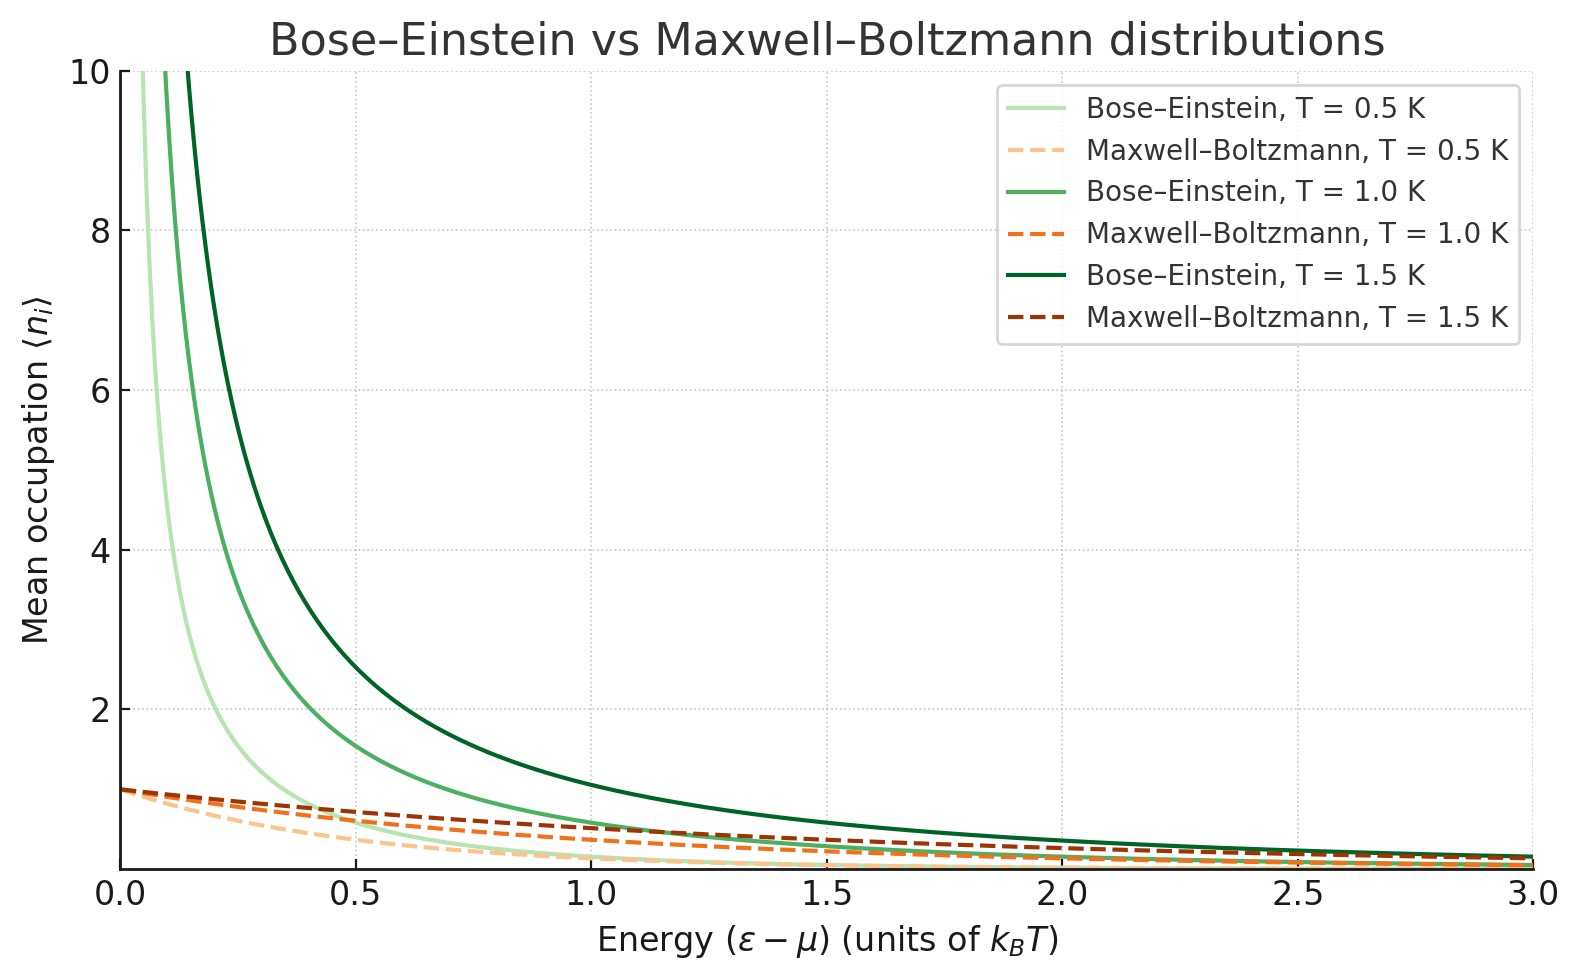
\includegraphics[scale= 0.2]{Chapters/Chapter_2/Images/2_BE_MB.jpg}
    \caption{Comparison between the Bose--Einstein and Maxwell--Boltzmann distributions at different temperatures.}
    \label{Figure 5 - BE_MB}
\end{figure}

\paragraph{Temperature dependence.}
The temperature dependence of the Bose--Einstein distribution is shown in Fig.~\ref{Figure 4 - Bose_Einstein_distribution} and further compared with the Maxwell--Boltzmann distribution at various temperatures in Fig.~\ref{Figure 5 - BE_MB}.
At high temperatures, the distribution is broad and relatively flat, resembling the classical Maxwell--Boltzmann form.  
As the temperature decreases, the distribution becomes increasingly peaked near the lowest energies.
When the critical temperature \( T_c \) is reached, a macroscopic number of particles condense into this state.

\section{Particle Number and Critical Density}

The total number of particles in a Bose gas is obtained by summing the average occupation of all single-particle states:
\begin{equation}
    N = \sum_i \langle n_i \rangle
      = \sum_i \frac{1}{e^{\beta(\varepsilon_i - \mu)} - 1}.
\end{equation}
In the thermodynamic limit\footnote{%
The thermodynamic limit refers to the situation in which the number of particles \(N\) and the volume \(V\) both tend to infinity while their ratio \(n = N/V\) remains constant.  
In this limit, discrete energy levels become quasi-continuous, allowing the replacement of the sum over states by an integral weighted by the density of states \(D(\varepsilon)\).%
}, this sum becomes an integral over the energy spectrum:
\begin{equation}
    N = \int_0^{\infty} D(\varepsilon)\, f(\varepsilon)\, d\varepsilon
      = \int_0^{\infty} \frac{D(\varepsilon)}{e^{\beta(\varepsilon - \mu)} - 1}\, d\varepsilon,
    \label{eq:N_integral}
\end{equation}
where \( f(\varepsilon) \) is the Bose–Einstein distribution and \( D(\varepsilon) \) is the \textit{density of states} (DOS), i.e. the number of single-particle states per unit energy interval.\\
For a three-dimensional gas of nonrelativistic particles confined in a volume \(V\), the quantization of momentum space yields\footnote{For a full derivation of the three-dimensional density of states \(D_{3D}\), see Appendix~\ref{app:BEC-derivation}, Section~\ref{density_of_states}.}:
\begin{equation}
    D_{3D}(\varepsilon) = \frac{V}{4\pi^2}
        \left(\frac{2m}{\hbar^2}\right)^{3/2} \varepsilon^{1/2}.
    \label{eq:DOS_3D}
\end{equation}
Substituting Eq.~\eqref{eq:DOS_3D} into Eq.~\eqref{eq:N_integral} and dividing by \(V\) yields the particle density:
\begin{equation}
\boxed{
    n = \frac{N}{V}
      = A \int_0^{\infty} d\varepsilon\, 
        \frac{\varepsilon^{1/2}}{e^{\beta(\varepsilon - \mu)} - 1},
    }
    \qquad
    A = \frac{m^{3/2}}{\sqrt{2}\pi^2\hbar^3}.
    \label{eq:n_integral_general}
\end{equation}

\subsection*{Critical Density}
To ensure a physically meaningful (non-negative) occupation number,
\[
\langle n_i \rangle = \frac{1}{e^{\beta(\varepsilon_i - \mu)} - 1} > 0,
\]
the denominator must remain positive, implying \( e^{\beta(\varepsilon - \mu)} > 1 \), i.e.\ \( \varepsilon > \mu \).  
In particular, for the lowest energy level (\(\varepsilon = 0\)), this requires
\[
\mu < 0.
\]

As the temperature decreases, \( \mu \) approaches zero from below, indicating that the lowest states become increasingly populated.  
When \( \mu \to 0^- \), a macroscopic occupation of the ground state begins to appear.  
In this limit, the maximum density that can be supported by the excited states is:
\begin{equation}
    n_c = A \int_0^{\infty} d\varepsilon\, 
           \frac{\varepsilon^{1/2}}{e^{\beta \varepsilon} - 1}.
    \label{eq:nc_integral}
\end{equation}

Introducing the dimensionless variable \( x = \varepsilon / (k_B T) \), we have:
\begin{equation}
    n_c = A (k_B T)^{3/2} 
          \int_0^{\infty} dx\, \frac{x^{1/2}}{e^x - 1}.
\end{equation}
The integral can be evaluated using the Gamma and Riemann zeta functions\footnote{For an introduction to and evaluation of this integral using the Gamma and Riemann zeta functions, see Appendix~\ref{app:BEC-derivation}, Section~\ref{appendix:gamma_riemann}.}:
\[
    \int_0^{\infty} \frac{x^{\alpha - 1}}{e^x - 1} dx = \Gamma(\alpha)\, \zeta(\alpha).
\]
For \( \alpha = 3/2 \), we obtain:
\begin{equation}
\boxed{
    n_c  = 
            A (k_B T)^{3/2}
          \,\Gamma\!\left(\tfrac{3}{2}\right)
          \,\zeta\!\left(\tfrac{3}{2}\right) = 
          \frac{m^{3/2}}{\sqrt{2}\pi^2\hbar^3} (k_B T)^{3/2}
          \,\Gamma\!\left(\tfrac{3}{2}\right)
          \,\zeta\!\left(\tfrac{3}{2}\right)
        }
          \label{eq:nc_result}
\end{equation}
It is convenient to introduce the thermal de Broglie wavelength
\begin{equation}
    \lambda_T = \frac{h}{\sqrt{2\pi m k_B T}},
\end{equation}
so that, using $\Gamma(3/2) = \sqrt{\pi}/2$, one finds
\begin{equation}
    n_c = \frac{1}{\lambda_T^3}\,\zeta\!\left(\tfrac{3}{2}\right),
\end{equation}
The quantity \(n_c\) thus represents the \textit{critical density} of particles that can be accommodated in the excited states at temperature \(T\).  
When the total particle density \(n\) exceeds this value, the surplus particles must accumulate in the ground state, giving rise to condensation.  
This formulation also reveals the physical significance of \(\lambda_T\):  
Bose–Einstein condensation occurs when the thermal wavelength becomes comparable to the mean interparticle spacing.

\subsection*{Critical Temperature and Condensate Fraction}
As discussed above, when the total density exceeds the critical value \(n_c\), the excess particles can no longer be accommodated in the excited states and therefore accumulate in the lowest energy level.
The total particle density can thus be expressed as:
\begin{equation}
    n = n_0 + n_{\mathrm{ex}},
    \label{eq:n_total}
\end{equation}
where \( n_0 \) represents the condensate density and \( n_{\mathrm{ex}} \) the density of particles occupying excited states.

\paragraph{Determination of the critical temperature.}
The critical temperature \(T_c\) corresponds to the point at which the density of thermally excited particles equals the total density, i.e.\ \(n = n_{\mathrm{ex}}(T_c) = n_c\).  
Using Eq.~\eqref{eq:nc_result} for \(n_c\) and the explicit form of \(A\) from Eq.~\eqref{eq:n_integral_general}, we have:
\[
n = \frac{m^{3/2}}{\sqrt{2}\pi^2\hbar^3} (k_B T_c)^{3/2}
          \,\Gamma\!\left(\tfrac{3}{2}\right)
          \,\zeta\!\left(\tfrac{3}{2}\right) = 
\frac{m^{3/2}(k_B T_c)^{3/2}}{2\sqrt{2}\,\pi^{3/2}\hbar^3}\,
      \zeta\!\left(\tfrac{3}{2}\right).
\]
Solving for \(T_c\):
\begin{equation}
(k_B T_c)^{3/2} = 
\frac{(2\pi\hbar^2)^{3/2}}{m^{3/2}}
\frac{n}{\zeta(3/2)}
\quad \Longrightarrow \quad
\boxed{
T_c = 
\frac{2\pi\hbar^2}{m k_B}
\left[\frac{n}{\zeta(3/2)}\right]^{2/3}
}\, .
\label{eq:Crit_T}
\end{equation}
This relation defines the transition temperature below which Bose--Einstein condensation occurs.

\paragraph{Derivation of the condensate fraction.}
For \( T < T_c \), the chemical potential remains fixed at \( \mu = 0 \), and the number of particles in excited states is:
\begin{equation}
    N_{\mathrm{ex}}(T) = V A (k_B T)^{3/2}
    \Gamma\!\left(\tfrac{3}{2}\right)
    \zeta\!\left(\tfrac{3}{2}\right),
    \label{eq:Nex_T}
\end{equation}
At \( T = T_c \), the total number of particles is:
\begin{equation}
    N = N_{\mathrm{ex}}(T_c)
      = V A (k_B T_c)^{3/2}
        \Gamma\!\left(\tfrac{3}{2}\right)
        \zeta\!\left(\tfrac{3}{2}\right).
    \label{eq:N_Tc}
\end{equation}
Dividing Eq.~\eqref{eq:Nex_T} by Eq.~\eqref{eq:N_Tc} gives the temperature dependence of the non-condensed fraction:
\[
    \frac{N_{\mathrm{ex}}(T)}{N}
    = \left(\frac{T}{T_c}\right)^{3/2}.
    \label{eq:Nex_fraction}
\]
Since the total number is \( N = N_0 + N_{\mathrm{ex}} \), the condensate population becomes:
\begin{equation}
\boxed{
    \frac{N_0}{N}
    = 1 - \left(\frac{T}{T_c}\right)^{3/2}.
    }
    \label{eq:condensate_fraction}
\end{equation}
This expression shows that the condensate fraction grows continuously from zero at \( T = T_c \) to unity as \( T \to 0 \).


\subsection*{Dimensionality Effects in BEC}
\label{Dimension_BEC}
The occurrence of Bose--Einstein condensation strongly depends on the dimensionality of the system and on the form of the single-particle dispersion relation.  
To illustrate this, we generalize the derivation of the critical density to lower dimensions and show explicitly that condensation cannot occur in two or one dimensions for nonrelativistic particles with quadratic dispersion.

\paragraph{Two-dimensional case.}
For a gas of nonrelativistic bosons confined in a square box of side \(L\), the single-particle energy levels are given by:
\[
    \varepsilon = \frac{\hbar^2}{2m}(k_x^2 + k_y^2),
\]
where: 
\[
k_x = \frac{\pi n_x}{L}, \qquad 
k_y = \frac{\pi n_y}{L}, \qquad 
n_x, n_y \in \mathbb{Z}.
\]
The density of states follows from counting the number of states within a ring of radius \(k\) and thickness \(dk\) in \(k\)-space.  
Each quantum state occupies an area \((2\pi/L)^2\), so the number of states between \(k\) and \(k+dk\) is: 
\[
  dN = \frac{L^2}{(2\pi)^2} \, 2\pi k\, dk  
\]
Since the particle energy is related to the wavevector by 
\(\varepsilon = \hbar^2 k^2 / (2m)\), we have: 
\[
    k\, dk = (m/\hbar^2)\, d\varepsilon \implies dN = \frac{L^2 m}{2\pi \hbar^2}\, d\varepsilon \implies 
D_{2\mathrm{D}}(\varepsilon) = \frac{dN}{d\varepsilon}
= \frac{mL^2}{2\pi \hbar^2}.
%\label{eq:DOS_2D}
\]
Unlike the three-dimensional case, the DOS is \textit{independent of energy}.  
The total number of particles occupying excited states is therefore:
\[
    N_{2\mathrm{D}} = \int_0^{\infty} 
    \frac{D_{2\mathrm{D}}\, d\varepsilon}
         {e^{\beta(\varepsilon - \mu)} - 1}
    = \frac{mL^2}{2\pi \hbar^2}
      \int_0^{\infty}
      \frac{d\varepsilon}{e^{\beta(\varepsilon - \mu)} - 1}.
    %\label{eq:N2D_integral}
\]
Expanding the Bose--Einstein factor using the geometric series
\[\frac{1}{e^{\beta(\varepsilon - \mu)} - 1} 
= \frac{e^{-\beta(\varepsilon - \mu)}}{1 - e^{-\beta(\varepsilon - \mu)}}
\]
and introducing the fugacity\footnote{The fugacity \( z = e^{\beta \mu} \) quantifies the effect of the chemical potential on the particle distribution.  
It measures the deviation of the system from the classical limit, where \( z \ll 1 \) corresponds to low densities (Maxwell--Boltzmann regime) and \( z \to 1^{-} \) signals the onset of quantum degeneracy.} \( z = e^{\beta \mu} \), we can express the integrand as
\[
    \frac{1}{e^{\beta(\varepsilon - \mu)} - 1}
    = \sum_{l=1}^{\infty} e^{-l\beta(\varepsilon - \mu)}
    = \sum_{l=1}^{\infty} z^l e^{-l\beta\varepsilon}.
\]
Substituting this expansion into the integral and integrating over the energy gives:
\[
    \int_0^{\infty} e^{-l\beta\varepsilon}\, d\varepsilon = \frac{1}{l\beta},
\]
which leads to:
\[
    N_{2\mathrm{D}} = 
    \frac{mL^2}{2\pi \hbar^2 \beta}
    \sum_{l=1}^{\infty} \frac{z^l}{l}.
\]
This summation represents a particular case of the \textit{Bose function}, defined in general\footnote{%
It appears frequently in the statistical description of Bose gases and reduces to the 
Riemann zeta function at the condensation point, $g_{\sigma}(1) = \zeta(\sigma).$  
} as
\begin{equation}
    g_{\sigma}(z) = \sum_{l=1}^{\infty} \frac{z^l}{l^{\sigma}},
    \qquad (|z|<1),
\end{equation}
In the present case, \(\sigma = 1\), the series can be summed in closed form using the identity:
\[
    \sum_{l=1}^{\infty} \frac{z^l}{l} = -\ln(1-z)\qquad (|z|<1).
\]
Therefore:
\[
    N_{2\mathrm{D}} 
    = \frac{mL^2}{2\pi \hbar^2 \beta}
      \sum_{l=1}^{\infty} \frac{z^l}{l}
    = -\frac{mL^2}{2\pi \hbar^2 \beta}\, \ln(1 - z).
\]
As the chemical potential approaches zero (\(\mu \to 0^{-}\), i.e.\ \(z=e^{\beta\mu}\to 1^{-}\)), the series diverges logarithmically. Hence the excited–state population:
\begin{equation}
    N_{2\mathrm{D}} = -\frac{mL^2}{2\pi \hbar^2 \beta}\,\ln(1-z)
\end{equation}
blows up. This logarithmic divergence indicates that long-range coherence cannot develop in a two-dimensional gas at any finite temperature. Thus, for massive bosons with quadratic dispersion in two dimensions,
\[
    \textit{BEC does not occur at any finite temperature \;} T.
\]

 This limitation becomes even more severe in one dimension, where the density of states further enhances the divergence.

\paragraph{One-dimensional case.}
In one dimension, the single-particle energy is:
\[
    \varepsilon = \frac{\hbar^2 k^2}{2m},
\]
and the number of states between \(k\) and \(k + dk\) in a box of length \(L\) is:
\[
    dN = \frac{L}{\pi} dk.
\]
Hence the density of states is:
\begin{equation}
    D_{1\mathrm{D}}(\varepsilon)
    = \frac{dN}{d\varepsilon}
    = \frac{L}{\pi \hbar} \sqrt{\frac{m}{2\varepsilon}}.
    \label{eq:DOS_1D}
\end{equation}
The total number of particles in excited states becomes:
\begin{equation}
    N_{1\mathrm{D}} = 
    \int_0^{\infty}
    \frac{D_{1\mathrm{D}}(\varepsilon)\, d\varepsilon}
         {e^{\beta(\varepsilon - \mu)} - 1}
    = \frac{L}{\pi \hbar} \sqrt{\frac{m}{2}}
      \int_0^{\infty}
      \frac{\varepsilon^{-1/2}\, d\varepsilon}
           {e^{\beta(\varepsilon - \mu)} - 1}.
\end{equation}
In the limit \(\mu \to 0\), the integrand behaves as \(\varepsilon^{-1/2}\) near \(\varepsilon = 0\), which causes the integral to diverge.  
As in the 2D case, all particles can be accommodated in excited states, and no condensation occurs at any finite temperature.

\paragraph{Dimensional Criterion for BEC.}\label{crit}
The absence of Bose--Einstein condensation in one and two dimensions reflects the dominance of low-energy fluctuations in reduced dimensionality.\\
For a dispersion relation of the form \(\varepsilon \propto K^s\), one can show that condensation occurs only if the integral
\begin{equation}
    \int_0^{\infty} \frac{\varepsilon^{d/s - 1}\, d\varepsilon}{e^{\beta(\varepsilon - \mu)} - 1}
    \label{convergence}
\end{equation}
converges when \(\mu \to 0\), which requires \(d/s > 1\).  
For quadratic dispersion $(s = 2)$, this condition is satisfied only for $d > 2$.
Therefore, true Bose–Einstein condensation is possible only in three or more dimensions.
In lower dimensions, quantum degeneracy effects can still appear, but they manifest as quasi-condensation rather than macroscopic occupation of a single quantum state.

The appearance of the condensate below the critical temperature $T_c$ signifies more than a simple redistribution of particles among energy levels.
It marks the emergence of a collective quantum state in which a macroscopic number of particles share the same single-particle wavefunction.
This coherence allows the entire system to be described by a single complex field, the \textit{macroscopic wavefunction} or \textit{order parameter}, whose magnitude reflects the condensate density and whose phase encodes its quantum coherence.\\
The Bose–Einstein condensation transition can thus be interpreted as a spontaneous breaking of the global $\mathrm{U}(1)$ phase symmetry associated with particle number conservation, a concept that will prove central in the description of superconductivity.\\
We now formalize this idea.

\section{Order Parameter and SSB}
We now formalize this idea by introducing the concept of the \textit{order parameter}, which characterizes the macroscopic coherence of the Bose–Einstein condensate.
Rather than describing the gas in terms of individual particle states, we can instead represent it through a single collective field that embodies both the amplitude and phase of the condensate.

\subsection*{Order Parameter}  
Below the critical temperature \(T_c\), a macroscopic number of particles occupy the same single-particle state \(\chi_0(\mathbf{r},t)\).  
The system can therefore be described by a collective complex field, the \textit{macroscopic wavefunction} or \textit{order parameter}:
\[
    \Psi(\mathbf{r},t) = \sqrt{N_0(t)}\, \chi_0(\mathbf{r},t),
    %\label{eq:order_parameter_def}
\]
where \(N_0(t)\) is the number of particles in the condensate.  
Since the single-particle wavefunction is normalized to unity, the normalization of \(\Psi\) satisfies
\[
    \int |\Psi(\mathbf{r},t)|^2\, d\mathbf{r} = N_0(t).
\]
The modulus \(|\Psi(\mathbf{r},t)|^2\) thus represents the local condensate density, while its phase encodes the global coherence of the quantum state.  \\
Conversely, above $T_c$, the phases of the individual particle states are random and uncorrelated, and the average macroscopic field vanishes, \(\Psi = 0\).

The order parameter therefore serves as a direct indicator of the phase transition:
\[
    \Psi(\mathbf{r},t) =
    \begin{cases}
        0, & T \geq T_c,\\[4pt]
        \neq 0, & T < T_c.
    \end{cases}
\]

A finite amplitude of $\Psi$ below $T_c$ signals the emergence of long-range coherence throughout the system, marking the onset of Bose–Einstein condensation.

\subsection*{Spontaneous Breaking of \texorpdfstring{$\mathrm{U}(1)$}{U(1)} Symmetry}

As discussed before, the formation of a Bose--Einstein condensate introduces a nonzero complex order parameter
\[
\Psi = \sqrt{n_0}\, e^{i\phi},
\]
whose modulus sets the condensate density and whose phase \(\phi\) defines its global coherence.  
While the phase itself has no direct influence on measurable quantities such as the density \(|\Psi|^2\), the act of choosing a definite value of \(\phi\) has deep physical significance: it marks the spontaneous breaking of a continuous symmetry.\\
Above the critical temperature \(T_c\), the gas has no preferred phase.  
Each particle’s wavefunction carries a random phase, and the macroscopic average vanishes, \(\Psi = 0\).  
In this regime, the system is invariant under global phase transformations,
\[
\Psi \;\to\; e^{i\theta}\Psi,
\]
so all phases are physically equivalent.\\
Below \(T_c\), however, a macroscopic number of particles condense into the same quantum state, and the order parameter acquires a finite value.  
Although the microscopic equations remain symmetric under the same phase rotations, the condensate itself must \emph{select} one specific phase \(\phi\) to establish coherence.  
The symmetry of the underlying laws is therefore preserved, but the symmetry of the macroscopic state is not, which is the essence of \textit{spontaneous symmetry breaking} (SSB).

The broken \(\mathrm{U}(1)\) phase symmetry introduces a new physical quantity, the global phase of the condensate, common to all particles and uniform throughout the system.  \\
Hence, Bose--Einstein condensation can be seen not only as the macroscopic occupation of the ground state, but as the spontaneous emergence of global phase order, a fundamental concept that will reappear in the description of superconductivity.

%==========================================================================

